% Chapter Template

\chapter{Definición del problema}

\label{Chapter5} % Change X to a consecutive number; for referencing this chapter elsewhere, use \ref{ChapterX}

%----------------------------------------------------------------------------------------
%	SECTION 1
%----------------------------------------------------------------------------------------

\section{Kaggle}

Kaggle es una plataforma donde se organizan competiciones de modelos predictivos o de aprendizaje automático sobre un problema real. Diferentes organizaciones plantean un problema un premio para el mejor modelo que lo resuelva, haciendo que miles de participantes prueben ideas diferentes y consigan puntos de vista que, en organizaciones tradicionales, un solo equipo no tendría.

En este trabajo se ha optado por la participación en uno de esos problemas, The Nature Conservancy Fisheries Monitoring.

\section{The Nature Conservancy Fisheries Monitoring}

En el océano pacífico, donde se captura más del 60\% del atún del mundo, tienen lugar prácticas de pesca irregular que amenazan a los ecosistemas marinos y a la estabilidad de la pesca mundial. The Nature Conservancy es una asociación que trabaja con organizaciones locales y globales para preservar las especies marinas de cara al futuro.

La principal idea para controlar la pesca y explotación de recursos marinos es el uso de cámaras en barcos, que ayudan a monitorizar las actividades pesqueras de estos. Aunque funciona muy bien como sistema de control, la cantidad de datos e imágenes generadas hace que sea muy costoso de procesar manualmente.

\begin{center}
  \makebox[\textwidth]{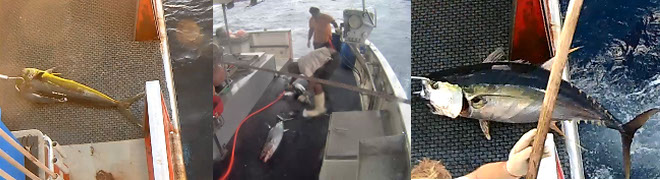
\includegraphics[width=\linewidth]{kaggle-competition-banner}}
\end{center}

La idea de este reto es desarrollar algoritmos que detecten y clasifiquen automáticamente especies de atunes, tiburones y otras especies que estos barcos pesqueros cazan. El hecho de que se pueda analizar este tipo de imágenes de una manera rápida y automática permitirá asignar recursos de una manera mucho más efectiva para el control de este tipo de actividades. (Cita: fisheries monitoring)

\section{Definición del problema}

El problema consiste en clasificar cada una de las imágenes de un conjunto de imágenes de barcos en una de las ocho categorías disponibles. Las imágenes suelen mostrar la cubierta de un barco donde puede aparecer un pez. En base al pez que aparezca hay que clasificarlo en una de las siguientes seis categorías:

\begin{center}
  \makebox[\textwidth]{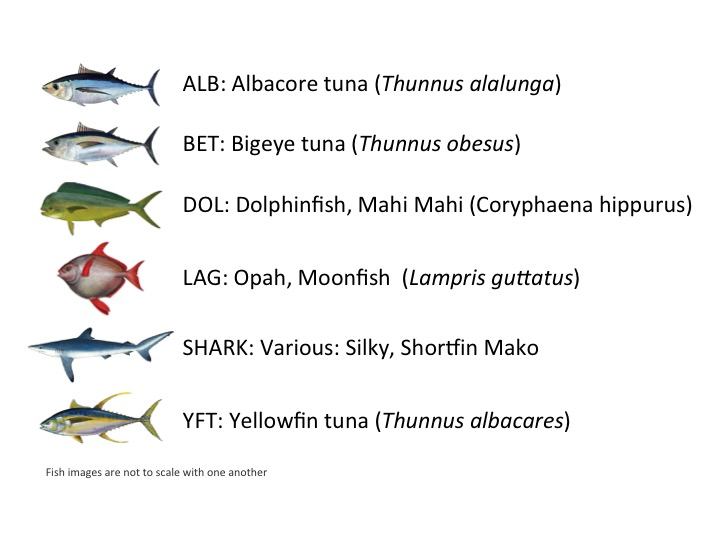
\includegraphics[width=\linewidth]{species-ref-key}}
\end{center}

En caso de que no aparezca ningún pez en la imagen, esta tendrá la categoría NOF (No Fish). Y si aparece un pez en la imagen pero no perteneciente a ninguna de las categorías mencionadas, la categoría será OTHER.

\[
  categories =
  \left[ALB, BET, DOL, LAG, SHARK, YFT, OTHER, NOF]
\]

\subsection{Conjunto de datos}

El conjunto de datos que se provee en el reto consta de tres elementos:

\begin{enumerate}
  \item{Conjunto de datos de entrenamiento: 3777 imágenes etiquetadas con una de las ocho categorías existentes.}
  \item{Conjunto de test y evaluación: 1000 imágenes sin etiquetar.}
  \item{Archivo de envío de prueba: Archivo CSV que muestra la estructura que debe tener el archivo con las soluciones}
\end{enumerate}

\subsection{Envío de la solución y evaluación}

Para el envío de la solución hace falta clasificar las 1000 imágenes del conjunto de evaluación, indicando la probabilidad de que caiga en cada una de las ocho categorías diferentes. En la tabla \ref{submission-sample} se muestra un ejemplo de las primeras filas del archivo CSV a enviar.

\begin{table}[]
\centering
\caption{Ejemplo del archivo de envío}
\label{submission-sample}
\begin{tabular}{lllllllll}
image          & ALB   & BET   & DOL   & LAG    & NoF   & OTHER & SHARK  & YFT  \\
img\_00005.jpg & 0.455 & 0.052 & 0.030 & 0.0173 & 0.123 & 0.079 & 0.046 & 0.194\\
img\_00007.jpg & 0.455 & 0.052 & 0.030 & 0.0173 & 0.123 & 0.079 & 0.046 & 0.194\\
img\_00009.jpg & 0.455 & 0.052 & 0.030 & 0.0173 & 0.123 & 0.079 & 0.046 & 0.194
\end{tabular}
\end{table}

El envío se evalúa usando multi-class logarithmic loss. Cada imagen ha sido etiquetada con una clase, pero es necesario enviar las probabilidades de cada clase para cada imagen. La formula final es:

\[
  logloss =
  - \frac{1}{N} \sum_{i=1}^N \sum_{j=1}^M y_{ij} \log \, p_{ij}
\],
 siendo N el número de imágenes en el conjunto de test, M el número de clases, $y_{ij}$ es 1 si la observación $i$ pertenece a la clase $j$ y 0 si no pertenece y $p_{ij}$ la probabilidad predecida de que el elemento $i$ pertenezca a la clase $j$.

 \subsecion{Leaderboard y fases de la competición}

 Existe una tabla donde se publican los resultados de los envíos de cada participante. Estos resultados están calculados solo con un subconjunto del conjunto de test, de esta manera se evita que los participantes puedan aprovechar un sobreajuste para subir en la clasificación.

La puntuación final vendrá determinada por la puntuación de todo el conjunto de test.

Esta manera de evaluar es algo bastante común en kaggle, sin embargo los organizadores de este reto en particular han decidido hacer un pequeño cambio a la hora de evaluar la puntuación.

\subsection{Doble fase de evaluación y envío}

La evaluación en este reto contará de dos partes. La primera, donde se entrenará el modelo, requiere (como ya se ha dicho) evaluar el conjunto de test de mil imágenes. La fecha límite para la entrega de modelos de esta primera fase es siete días antes de la finalización del reto. Será necesario enviar el CSV con las predicciones y el modelo usado.

Una vez finalice la primera fase, un segundo conjunto de test de muchas más imágenes será hecho público. Este conjunto de test deberá ser evaluado con el modelo generado en la fase anterior, siendo razón de descalficación modificar el modelo. Todos los participantes que no envíen la predicción de la segunda fase serán eliminados del reto.
